\documentclass[12pt]{article}
\usepackage{preamble}
\usepackage{misccorr}

\pagestyle{fancy}
\fancyhead[LO,LE]{Специальные разделы \\ высшей математики}
\fancyhead[CO,CE]{01.03.2024}
\fancyhead[RO,RE]{Лекции Далевской О. П.}


\begin{document}
    \textit{\vspace{3mm}
\textit{Nota}: } Изоморфизм $E^n \rightarrow E^{\prime n}$ позволяет переносить свойства скалярного произведения
    из одного в другое пространство

    \vspace{3mm}
\textit{Ex}: $\|x + y\| \leq \|x\| + \|y\|$ - арифметические векторы со скалярным произведением $\displaystyle (x, y) = \Sigma^n_{i=1} x_i y_i$

    $E^{\prime n} \in C_{[a;b]}$ со скалярным произведением $\displaystyle (f, g) = \int^b_a f * g dx$

    $\displaystyle \sqrt{\int^b_a (f * g)^2 dx} \leq \sqrt{\int^b_a f^2 dx} + \sqrt{\int^b_a g^2 dx}$

    \textbf{Задача о перпендикуляре}

    Постановка: Нужно опустить перпендикуляр из точки пространства $E^n$ на подпространство $G$

    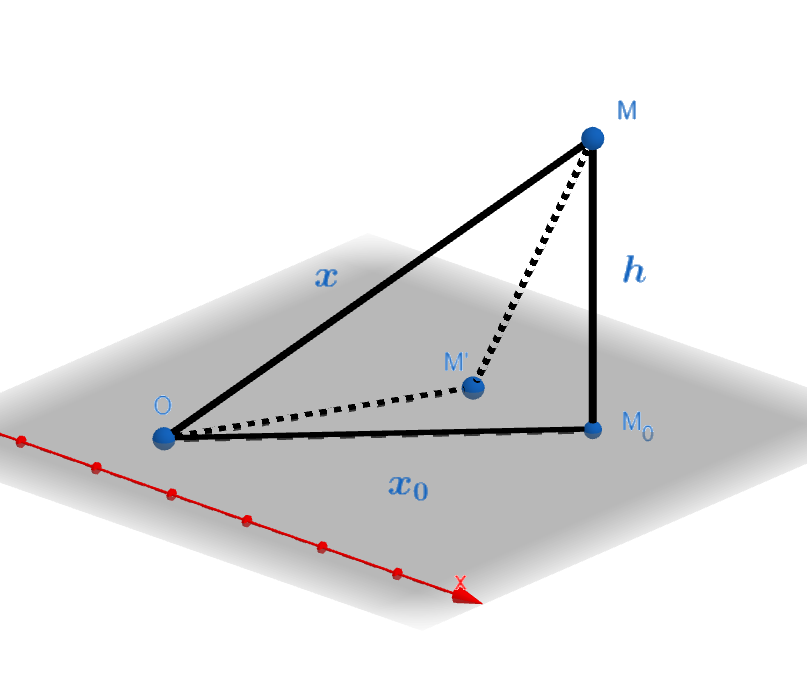
\includegraphics[height=90mm]{images/specsec_2024_03_01_1}

    Точка $M$ - конец вектора $x$ в пространстве $E^n$.
    Нужно найти $M_0$ (конец вектора $x_0$, проекции $x$ на $G$)

    \[x_0 + h = x\]

    где $h \perp G$. Правда ли что, длина перпендикулярного вектора $h$ - минимальная длина от точки $M$ до $G$?

    \textit{\vspace{3mm}
\textit{Th}: } $h \perp G, x_0 \in G, x = x_0 + h$. Тогда $\forall x^\prime \in G (x^\prime \neq x_0) \ \ \|x - x^\prime\| > \|x - x_0\|$

    $\Box \|x - x^\prime\| = \|x - x_0 + x_0 - x^\prime\| \stackrel{\text{по теореме Пифагора}}{====} \|x - x_0\| + \|x_0 - x^\prime\| = \|h\| + \|x_0 - x^\prime\| > \|x - x_0\|$

    \vspace{5mm}

    \textit{\vspace{3mm}
\textit{Nota}: } $x_0$ называется ортогональной проекцией, возникает вопрос о ее вычислении (так находятся основания перпендикуляров)

    \vspace{5mm}

    \textit{Алгоритм:} $x_0 = \lambda_1 e_1 + \lambda_2 e2 + \dots + \lambda_k + e_k$, $\{e_i\}^k_{i=1}$ - базис $G$ (необязательно ортонормированный)

    Дан вектор $x$, пространство $G$, нужно найти $\lambda_i$

    $h = x - x_0$, $h \perp G \quad  (h, e_i) \stackrel{h \perp e_i \ \forall i}{=} 0$

    $(x - x_0, e_i) = (x, e_i) - (x_0, e_i) = 0$

    $(x, e_i) = (x_0, e_i)$

    Тогда $\forall i \quad (x_0, e_i) = (\lambda_1 e_1 + \dots + \lambda_k e_k, e_i) = \lambda_1 (e_1, e_i) + \dots + \lambda_k (e_k, e_i)$ - $(e_k, e_i)$ - числа, а $\lambda_i$ - неизвестные

    \vspace{5mm}
    \textbf{
    Получили СЛАУ:}

    $\begin{array}{|cccc|}
    (e_1, e_1) & (e_1, e_2) & \ldots & (e_1, e_k)\\
    \ldots & \ldots & \ldots & \ldots\\
    (e_k, e_1) & (e_k, e_2) & \ldots & (e_k, e_k)\\
    \end{array} \times \begin{array}{|c|}
    \lambda_1\\
    \ldots\\
    \lambda_k \\
    \end{array} = \Gamma \times \begin{array}{|c|}
    \lambda_1\\
    \ldots\\
    \lambda_k \\
    \end{array} = \begin{array}{|c|}
    (x,e_1)\\
    \ldots\\
    (x,e_k) \\
    \end{array}$

    \textit{\vspace{3mm}
\textit{Nota}:} В матрице $\Gamma$ нет нулевых строк, так как $e_i$ - бизисная и по крайней мере $e_i^2 \neq 0$

    Таким образом по теореме Крамера $\exists! (\lambda_1, \dots, \lambda_k)$

    \textit{\vspace{3mm}
\textit{Def}:} Матрица $\Gamma = {(e_i, e_j)}_{i, j = 1\dots k}$ называют матрицей Грама

    $\Gamma = I = \begin{array}{|ccc|}
    1 & 0 & \ldots\\
    0 & 1 & \ldots\\
    \ldots & \ldots & 1\\
    \end{array}$, если базис ортонормированный

    Далее, $I$ - единичная матрица Грама

    \textit{\vspace{3mm}
\textit{Nota}:} Тогда $I \times \begin{array}{|c|}
    \lambda_1\\
    \ldots\\
    \lambda_k \\
    \end{array} = \begin{array}{|c|}
    \lambda_1\\
    \ldots\\
    \lambda_k \\
    \end{array} = \begin{array}{|c|}
    (x,e_1)\\
    \ldots\\
    (x,e_k) \\
    \end{array}$

    \vspace{5mm}

    \textbf{Приложения задачи о перпендикуляре}

    1) Метод наименьших квадратов

    В качестве простейшей модели зависимости $y = y(x)$ берем линейную функцию $y = \lambda x$

    Ищем минимально отстоящую прямую от данных $(x_i, y_i)$, то есть ищем $\lambda$

    Определим расстояние (в этом методе) как $\displaystyle \sigma^2 = \Sigma^n_{i=1} (y_i - y_{0i})^2 = \Sigma^n_{i=1} (y_i - \lambda x_i)^2$ - минимизируем

    Таким образом, ищем $y_0$ (ортог. проекция) такое, что $(y - y_0)^2 = \sigma^2$ - минимальное

    Если $y_0 = \lambda_1 x_1 + \dots + \lambda_k x_k$, где $x_i$ - набор измерений для $i$-ой точки

    Рассмотрим $y_0$ как разложение по базису $\{x_i\}$

    \vspace{5mm}

    2) Многочлен Фурье

    $\displaystyle P(t) = \frac{a_0}{2} + a_1 cos t + b_1 sin t + \dots a_n cos nt + b_n sin nt$ - линейная комбинация

    Функции ${1, cos t, sin t, \dots, cos nt, sin nt}$ - ортогональны

    Задача в том, чтобы для функции $f(t)$, определенной на отрезке $[0;2\pi]$ найти минимально отстоящий многочлен $P(t)$ при том,
    что расстояние определяется как $\displaystyle \sigma^2 = \int_0^{2\pi} (f(t) - P(t))^2 dt$

    Нужно найти $a_i$ и $b_i$ - обычные скалярные произведения $\displaystyle a_i = k \int_0^{2\pi} f(t) cos(it) dt$, $\displaystyle b_i = m \int_0^{2\pi} f(t) sin(it) dt$ ($k, m$ - нормирующие множители)

    \clearpage

    \textbf{2. Линейный оператор (линейное отображение, линейный функционал, линейное преображение)}

    \textbf{2.1 Определение}

    \textit{Линейный оператор} - это отображение $V^n \stackrel{\mathcal{A}}{\Longrightarrow} W^m$

    ($V^n, W^m$ - линейные пространства размерности $n \neq m$ в общем случае),

    которое $\forall x \in V^n$ сопоставляет один какой-либо $y \in W^m$ и

    $\mathcal{A} (\lambda x_1 + \mu x_2) = \lambda \mathcal{A} x_1 + \mu \mathcal{A} x_2 = \lambda y_1 + \mu y_2$

    \vspace{3mm}

    \textit{\vspace{3mm}
\textit{Nota}:} Заметим, что если 0 представим как $0 * x$, где $x \neq 0$, то

    $\mathcal{A}(0) = \mathcal{A}(0 * x) = 0 * \mathcal{A}x \stackrel{0 * y}{=} 0$

    \textit{\vspace{3mm}
\textit{Nota}:} Если $V = W$, то $\mathcal{A}$ называют линейным преобразованием, но далее будем рассматривать в основном операторы $\mathcal{A}: \ \ V \rightarrow V$, $\mathcal{A}: \ \ V^n \rightarrow W^n$

    \vspace{3mm}

    \textit{\vspace{3mm}
\textit{Ex}.1:} $V = \Real^2$ - пространство направленных отрезков

    $\mathcal{A}: V \leftarrow V$

    $\mathcal{A}x = y = \lambda y_1 + \mu y_2$ для таких $\mathcal{A}$ как сдвиг, поворот, гомотетия, симметрия

    \textit{\vspace{3mm}
\textit{Ex}.2:} $V^n = W^m$, где $m < n$

    $\mathcal{A}$ - оператор проектирования (убедиться, что он линейный)

    \textit{\vspace{3mm}
\textit{Ex}.3:} $V^n$ - пространство числовых строк длины $n$

    $\mathcal{A}: V^n \leftarrow V^n$

    $x = (x_1, \dots, x_n), y = (y_1, \dots, y_n)$

    $\mathcal{A}x = y : \begin{array}{|ccc|}
    a_{11} & \ldots & a_{1n}\\
    \vdots & \ddots & \vdots\\
    a_{n1} & \ldots & a_{nn}\\
    \end{array}x = y$

    \vspace{5mm}

    \textbf{2.2. Действия с операторами}

    \textit{\vspace{3mm}
\textit{Def}:} $\mathcal{A}\mathcal{B}: V \rightarrow W$

    \begin{enumerate}
        \item $(\mathcal{A} + \mathcal{B})x \stackrel{def}{=} \mathcal{A}x + \mathcal{B}x$ - определение суммы $\mathcal{A} + \mathcal{B} = \mathcal{C}$
        \item $(\lambda\mathcal{A})x \stackrel{def}{=} \lambda(\mathcal{A}x)$ - $\lambda\mathcal{A} = \mathcal{D}$
    \end{enumerate}

    \textit{\vspace{3mm}
\textit{Nota}:} Сформируем линейное пространство из операторов $\mathcal{A}: V \rightarrow W$

    \begin{enumerate}
        \item Ассоциативность сложения (очевидно)
        \item Коммутативность (очевидно)
        \item Нейтральный элемент $\mathcal{O}x = 0$
        \item Противоположный: $-\mathcal{A} = (-1) * A$
        \item \dots \textit{LAB}
    \end{enumerate}

    \textit{\vspace{3mm}
\textit{Def}:} $\mathcal{I}$ - тождественный - $\forall x \in V \ \ \mathcal{I}x = x$

\end{document}
